\chapter{Mutações e variação genética}\label{ch:g11:mutations}

Nasce uma criança sem pigmento nenhum --- cabelo branco, pele clara,
olhos que não suportam luz forte --- de dois pais comuns, de uma
família sem história da condição. Uma colônia de bactérias que nunca
encontrou um antibiótico contém, entre cem milhões de \omterm{def:g10:cells-common-unit:cell}{células}, algumas
que já resistem a ele. Um jardineiro encontra um único ramo de uma
roseira com flores de outra cor. Em cada caso uma sequência de \omterm{def:g10:universal-dna:information}{DNA}
mudou, uma vez, numa \omterm{def:g10:cells-common-unit:cell}{célula}; e em cada caso a mudança passa a ser
copiada fielmente. Este capítulo trata dessas mudanças: o que elas são,
de onde vêm, como a \omterm{def:g10:cells-common-unit:cell}{célula} as limita, e por que a vida depende de elas
nunca pararem de todo.

\section{O que é uma mutação}

\begin{definition}[Mutação]\label{def:g11:mutations:mutation}
Uma \emph{mutação}\index{mutação} é uma mudança na sequência de
\omterm{def:g10:universal-dna:nucleotide}{nucleotídeos} de uma molécula de \omterm{def:g10:universal-dna:information}{DNA}, transmitida aos descendentes da
\omterm{def:g10:cells-common-unit:cell}{célula} em que ela acontece. As mais comuns são as
\emph{mutações pontuais}, que afetam um ou poucos \omterm{def:g10:universal-dna:nucleotide}{nucleotídeos}:
\begin{itemize}
  \item a \emph{substituição}: um \omterm{def:g10:universal-dna:nucleotide}{nucleotídeo} trocado por outro;
  \item a \emph{inserção}: um ou mais \omterm{def:g10:universal-dna:nucleotide}{nucleotídeos} acrescentados;
  \item a \emph{deleção}: um ou mais \omterm{def:g10:universal-dna:nucleotide}{nucleotídeos} retirados.
\end{itemize}
Mudanças maiores --- um segmento duplicado, invertido, deslocado, ou um
\omterm{def:g11:cell-cycle-mitosis:chromosome}{cromossomo} inteiro ganho ou perdido --- também são mutações.
\end{definition}

\begin{omfigure}
\begin{tikzpicture}[font=\small\ttfamily]
  \tikzset{seq/.style={anchor=west}}
  \node[seq] at (0,0) {original\ \ \ \ \ \ ATG GCT TAC GGA TCC};
  \node[seq] at (0,-0.8) {substituição\ \ ATG GCT T\textcolor{omThm}{\textbf{G}}C GGA TCC};
  \node[seq] at (0,-1.6) {inserção\ \ \ \ \ \ ATG GCT TA\textcolor{omThm}{\textbf{A}} CGG ATC C};
  \node[seq] at (0,-2.4) {deleção\ \ \ \ \ \ \ ATG GCT T\textcolor{omThm}{\textbf{\_}}C GGA TCC};
  \node[seq, font=\small] at (7.9,-0.8) {uma letra trocada};
  \node[seq, font=\small] at (7.9,-1.6) {uma letra a mais: tudo o que segue se desloca};
  \node[seq, font=\small] at (7.9,-2.4) {uma letra a menos: tudo o que segue se desloca};
\end{tikzpicture}

{\small Três mutações pontuais da mesma sequência (as letras estão
agrupadas de três em três por uma razão explicada no
\cref{ch:g11:gene-expression}). Uma substituição muda uma posição; uma
inserção ou uma deleção desloca tudo o que vem depois.}
\end{omfigure}

\begin{proposition}[Onde as mutações acontecem, e a quem]\label{prop:g11:mutations:where}
Uma \omterm{def:g11:mutations:mutation}{mutação} que acontece numa \omterm{def:g10:cells-common-unit:cell}{célula} do corpo (uma
\emph{\omterm{def:g11:mutations:mutation}{mutação} somática}) é passada apenas aos descendentes daquela
\omterm{def:g10:cells-common-unit:cell}{célula}: no máximo uma mancha de tecido, num só indivíduo. Uma \omterm{def:g11:mutations:mutation}{mutação}
numa \omterm{def:g10:cells-common-unit:cell}{célula} germinativa --- um gameta ou uma das precursoras dele --- é
passada à descendência concebida a partir dela e a todas as \omterm{def:g10:cells-common-unit:cell}{células}
dessa descendência: uma \emph{\omterm{def:g11:mutations:mutation}{mutação} germinativa} é o único tipo que
entra na hereditariedade da \omterm{def:g10:biodiversity-scales:species}{espécie}. O ramo estranho da roseira é
somático; a condição da criança sem pigmento veio de uma \omterm{def:g11:mutations:mutation}{mutação}
germinativa em algum ancestral, carregada em silêncio por gerações.
\end{proposition}
\admitted

\begin{example}[A frequência da mutação]\label{ex:g11:mutations:frequency}
A replicação deixa cerca de um erro por $10^9$ \omterm{def:g10:universal-dna:nucleotide}{nucleotídeos}
(\cref{ch:g11:dna-replication}). Um \omterm{def:g10:universal-dna:gene}{gene} de $\num{3000}$ pares de bases
é, portanto, copiado com erro cerca de uma vez a cada
$\num{300000}$ replicações; um ser humano, cujo genoma é copiado umas
$10^{16}$ vezes ao longo da vida, acumula mutações em cada \omterm{def:g10:universal-dna:gene}{gene} em
muitas \omterm{def:g10:cells-common-unit:cell}{células}. Cada criança nasce com umas 60 mutações novas que
nenhum dos pais carregava --- quase todas nos 98\% do genoma que não
são \omterm{def:g10:universal-dna:gene}{genes}.
\end{example}

\section{Causas: espontâneas e induzidas}

\begin{proposition}[Mutações espontâneas]\label{prop:g11:mutations:spontaneous}
As mutações surgem em toda \omterm{def:g10:cells-common-unit:cell}{célula}, na ausência de qualquer agente
externo: dos raros pareamentos errados que escapam à conferência da
polimerase, e da própria instabilidade química do \omterm{def:g10:universal-dna:information}{DNA}, cujas bases são
danificadas milhares de vezes por dia por \omterm{def:g10:cells-common-unit:cell}{célula} pela água e pelas
moléculas reativas do \omterm{def:g10:cell-metabolism:metabolism}{metabolismo} comum. Essas
\emph{mutações espontâneas} são \emph{aleatórias}: elas acontecem em
qualquer posição, a uma taxa que não depende de a mudança ser útil ou
não à \omterm{def:g10:cells-common-unit:cell}{célula}.
\end{proposition}
\begin{proof}[Evidências]
Lederberg (1952) espalhou numa placa bactérias nunca expostas a um
antibiótico, deixou que crescessem em colônias, depois pressionou uma
almofada de veludo sobre a placa e carimbou a marca dela --- as mesmas
colônias nas mesmas posições --- em várias placas contendo o
antibiótico. As poucas colônias resistentes apareceram nas
\emph{mesmas posições} em todas as placas com antibiótico. Como elas
vinham das mesmas colônias da placa original, que nunca tinha visto o
antibiótico, a \omterm{def:g11:mutations:mutation}{mutação} de resistência existia antes da exposição: o
antibiótico a revelou e não a causou. As mutações tinham acontecido ao
acaso durante o crescimento das colônias, sem consideração pela
utilidade futura delas.
\end{proof}

\begin{omfigure}
\begin{tikzpicture}[font=\small, >=Stealth]
  \tikzset{plate/.style={draw, thick, circle, minimum size=2.4cm, fill=omDef!6}}
  \node[plate] (p0) at (0,0) {};
  \foreach \x/\y in {-0.6/0.5, 0.3/0.7, -0.2/-0.2, 0.7/-0.1, -0.7/-0.6, 0.4/-0.7, 0.0/0.25, -0.35/0.85}
    \fill[omDef!60] (\x,\y) circle (2.2pt);
  \fill[omThm] (0.3,0.7) circle (2.6pt); \fill[omThm] (-0.7,-0.6) circle (2.6pt);
  \node[anchor=north, align=center] at (0,-1.35) {placa original,\\ sem antibiótico};
  \node[draw, fill=gray!25, minimum width=2.4cm, minimum height=0.35cm] (v) at (3.6,0) {veludo};
  \draw[->, thick] (1.3,0) -- (v.west);
  \node[plate, fill=omProp!8] (p1) at (7.0,1.5) {};
  \node[plate, fill=omProp!8] (p2) at (7.0,-1.5) {};
  \draw[->, thick] (v.east) -- (5.7,1.2);
  \draw[->, thick] (v.east) -- (5.7,-1.2);
  \fill[omThm] (7.3,2.2) circle (2.6pt); \fill[omThm] (6.3,0.9) circle (2.6pt);
  \fill[omThm] (7.3,-0.8) circle (2.6pt); \fill[omThm] (6.3,-2.1) circle (2.6pt);
  \node[anchor=west, align=left] at (8.3,1.5) {placa com antibiótico:\\ as mesmas duas posições};
  \node[anchor=west, align=left] at (8.3,-1.5) {placa com antibiótico:\\ as mesmas duas posições};
\end{tikzpicture}

{\small A réplica em placa. As colônias crescidas sem antibiótico são
carimbadas em placas com antibiótico. As colônias resistentes (em
vermelho) aparecem em posições idênticas em todas as réplicas: a
resistência existia nas colônias originais, antes de qualquer contato
com o medicamento.}
\end{omfigure}

\begin{definition}[Mutágeno]\label{def:g11:mutations:mutagen}
Um \emph{mutágeno}\index{mutágeno} é um agente físico ou químico que
eleva a taxa de \omterm{def:g11:mutations:mutation}{mutação} danificando o \omterm{def:g10:universal-dna:information}{DNA}. A luz ultravioleta solda
timinas vizinhas uma à outra numa fita; os raios X e a radioatividade
rompem as fitas; substâncias químicas como o benzopireno da fumaça do
tabaco ou a aflatoxina de grãos mofados se prendem às bases e distorcem
a hélice. Uma \omterm{def:g10:cells-common-unit:cell}{célula} exposta a um mutágeno carrega
\emph{mutações induzidas} além das espontâneas dela --- ainda em
posições aleatórias, apenas em maior número.
\end{definition}

\begin{example}[Ultravioleta em levedura]\label{ex:g11:mutations:uv}
\omterm{def:g10:cells-common-unit:cell}{Células} de levedura espalhadas em placas e expostas à luz ultravioleta
por tempos crescentes: depois de \qty{10}{s} metade das \omterm{def:g10:cells-common-unit:cell}{células} deixa
de formar colônia, depois de \qty{20}{s} um quarto, depois de
\qty{30}{s} um oitavo --- cada dose reduz os sobreviventes à metade.
Entre os sobreviventes, a proporção de colônias com uma característica
visivelmente mudada (cor, forma, incapacidade de crescer num certo
açúcar) sobe de uma em um milhão para uma em mil. A lâmpada mata
danificando o \omterm{def:g10:universal-dna:information}{DNA} além do reparo, e provoca \omterm{def:g11:mutations:mutation}{mutação} danificando-o um
pouco aquém disso.
\end{example}

\begin{omfigure}
\begin{tikzpicture}
\begin{axis}[
  width=0.86\linewidth, height=5.6cm,
  axis x line=bottom, axis y line=left,
  xmin=0, xmax=65, ymin=0, ymax=110,
  xlabel={exposição ao ultravioleta (s)}, ylabel={sobreviventes (\%)},
  xlabel style={font=\small, at={(axis description cs:0.5,-0.12)}, anchor=north},
  ylabel style={font=\small},
  tick label style={font=\small}, xtick={0,10,20,30,40,50,60}, ytick={0,25,50,75,100},
  legend style={at={(0.97,0.95)}, anchor=north east, font=\small, draw=none},
  legend cell align=left,
]
\addplot[thick, omDef, mark=*, mark size=1.5pt] coordinates
  {(0,100) (10,50) (20,25) (30,12.5) (40,6.3) (50,3.1) (60,1.6)};
\addplot[thick, omThm, dashed, mark=square*, mark size=1.5pt] coordinates
  {(0,100) (10,10) (20,1) (30,0.1) (40,0.01)};
\legend{levedura normal, levedura sem uma enzima de reparo}
\end{axis}
\end{tikzpicture}

{\small Sobrevivência de \omterm{def:g10:cells-common-unit:cell}{células} de levedura em função da exposição ao
ultravioleta. As \omterm{def:g10:cells-common-unit:cell}{células} normais perdem metade do número delas a cada
\qty{10}{s}; uma linhagem incapaz de reparar o dano do ultravioleta
perde nove décimos a cada \qty{10}{s}. A diferença é o trabalho do
reparo.}
\end{omfigure}

\begin{omfigure}
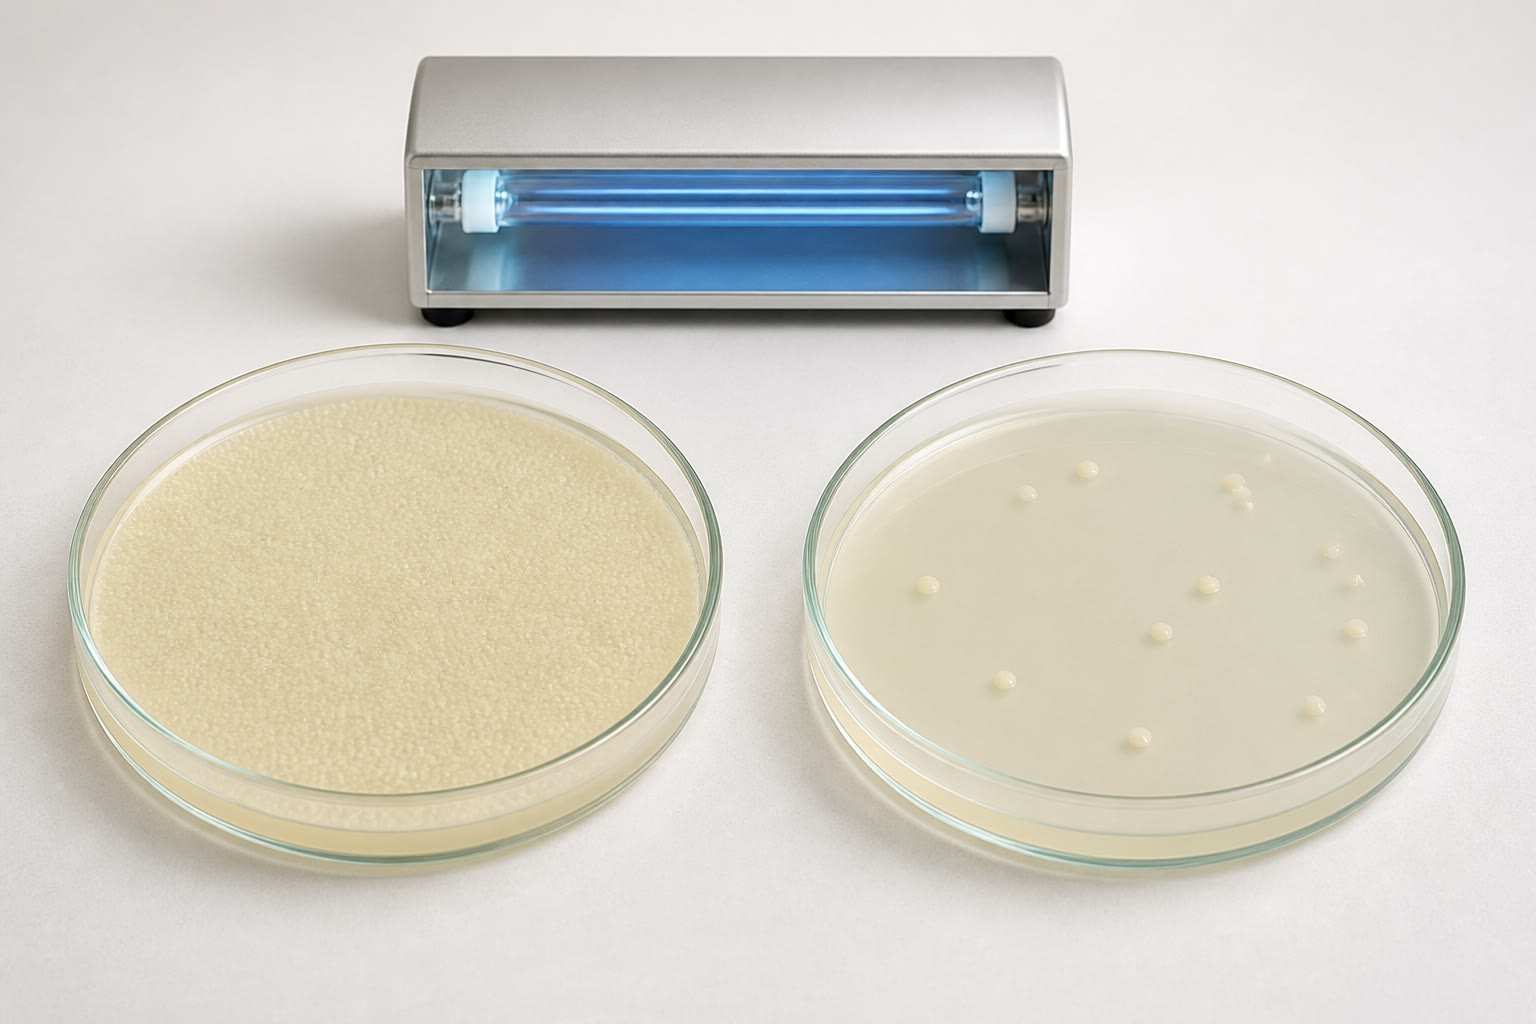
\includegraphics[width=0.6\linewidth]{images/book2/ai/g11-mutation-uv-plates.jpg}

{\small Duas placas semeadas com as mesmas bactérias. À esquerda: sem
exposição, um tapete contínuo. À direita: depois da exposição ao
ultravioleta, só as \omterm{def:g10:cells-common-unit:cell}{células} cujo dano no \omterm{def:g10:universal-dna:information}{DNA} foi reparado a tempo
cresceram em colônias.}
\end{omfigure}

\section{A célula reage: o reparo}

\begin{proposition}[O reparo do DNA]\label{prop:g11:mutations:repair}
Uma \omterm{def:g10:cells-common-unit:cell}{célula} sofre dezenas de milhares de lesões no \omterm{def:g10:universal-dna:information}{DNA} por dia e quase
não guarda nenhuma delas: sistemas de \omterm{def:g10:cell-metabolism:metabolism}{enzimas} dedicados patrulham a
\omterm{prop:g10:universal-dna:helix}{dupla-hélice}, reconhecem uma base danificada ou mal pareada, recortam o
segmento defeituoso de uma fita e o reconstroem usando a outra fita
como molde --- a \omterm{prop:g10:universal-dna:helix}{complementaridade} do \cref{ch:g10:universal-dna} mais
uma vez. Uma lesão só vira \omterm{def:g11:mutations:mutation}{mutação} se escapar do reparo antes de a
replicação seguinte a copiar. O reparo é a razão de a taxa de \omterm{def:g11:mutations:mutation}{mutação}
ser $10^{-9}$ e não $10^{-5}$.
\end{proposition}
\begin{proof}[Evidências]
As pessoas com a condição hereditária chamada xeroderma pigmentoso não
têm uma das \omterm{def:g10:cell-metabolism:metabolism}{enzimas} que retiram o dano do ultravioleta. A pele delas,
exposta à luz do dia comum, desenvolve cânceres mil vezes mais vezes
que a pele normal e desde a primeira infância; protegida do sol, ela é
normal. O mesmo ultravioleta, as mesmas lesões --- mas sem o reparo as
lesões ficam, e as mutações se acumulam nos \omterm{def:g10:universal-dna:gene}{genes} que controlam a
divisão celular (\cref{ch:g11:cancer}). Linhagens de levedura e de
bactérias sem \omterm{def:g10:cell-metabolism:metabolism}{enzimas} de reparo mostram a mesma hipersensibilidade no
laboratório.
\end{proof}

\begin{omfigure}
\begin{tikzpicture}[font=\small, >=Stealth,
  b/.style={draw, rounded corners, align=center, text width=2.6cm, minimum height=1.1cm}]
  \node[b, fill=omProp!15] (a) at (0,0) {o ultravioleta solda\\ dois T vizinhos};
  \node[b, fill=omDef!12] (bx) at (3.4,0) {enzimas de reparo\\ detectam a distorção};
  \node[b, fill=omDef!12] (c) at (6.8,0) {segmento danificado\\ recortado de uma fita};
  \node[b, fill=omDef!12] (d) at (10.2,0) {lacuna refeita com\\ a fita intacta};
  \draw[->] (a) -- (bx); \draw[->] (bx) -- (c); \draw[->] (c) -- (d);
  \node[b, fill=omThm!12] (e) at (3.4,-2.0) {a replicação copia\\ a lesão};
  \node[b, fill=omThm!12] (f) at (6.8,-2.0) {uma mutação, agora\\ permanente};
  \draw[->] (a.south) |- node[pos=0.25, left, font=\scriptsize, align=right] {se não for reparada\\ a tempo} (e.west);
  \draw[->] (e) -- (f);
\end{tikzpicture}

{\small A corrida entre o reparo e a replicação. Uma lesão recortada e
refeita a partir da outra fita não deixa rastro; uma lesão ainda
presente quando a forquilha passa é copiada para dentro da sequência e
vira uma \omterm{def:g11:mutations:mutation}{mutação}.}
\end{omfigure}

\section{Consequências de uma mutação}

\begin{proposition}[Da sequência ao fenótipo]\label{prop:g11:mutations:consequences}
Uma \omterm{def:g11:mutations:mutation}{mutação} transforma um \omterm{def:g10:universal-dna:gene}{alelo} num \omterm{def:g10:universal-dna:gene}{alelo} novo. O efeito dela depende
de onde ela cai e do que ela faz com a \omterm{def:g10:chemistry-of-life:families}{proteína} que o \omterm{def:g10:universal-dna:gene}{gene} codifica (o
\cref{ch:g11:gene-expression} dá as regras):
\begin{itemize}
  \item fora de qualquer \omterm{def:g10:universal-dna:gene}{gene}, ou numa posição que não muda a
        \omterm{def:g10:chemistry-of-life:families}{proteína}: \emph{sem efeito} --- a grande maioria;
  \item dentro de um \omterm{def:g10:universal-dna:gene}{gene}, mudando um \omterm{def:g10:chemistry-of-life:families}{aminoácido}: uma \omterm{def:g10:chemistry-of-life:families}{proteína} que
        funciona um pouco diferente, ou não funciona, ou às vezes
        funciona melhor;
  \item dentro de um \omterm{def:g10:universal-dna:gene}{gene}, deslocando ou truncando a mensagem: em
        geral uma \omterm{def:g10:chemistry-of-life:families}{proteína} que não funciona.
\end{itemize}
Se uma \omterm{def:g10:chemistry-of-life:families}{proteína} mudada é prejudicial, neutra ou útil depende do
ambiente: o mesmo \omterm{def:g10:universal-dna:gene}{alelo} de um \omterm{def:g10:universal-dna:gene}{gene} da hemoglobina é um fardo numa
região sem malária e uma proteção onde a malária existe.
\end{proposition}
\admitted

\begin{example}[Pigmento perdido, pigmento conservado]\label{ex:g11:mutations:pigment}
O pigmento melanina é fabricado por uma \omterm{def:g10:cell-metabolism:metabolism}{enzima}. São conhecidas dezenas
de mutações diferentes do \omterm{def:g10:universal-dna:gene}{gene} dela, cada uma produzindo uma \omterm{def:g10:cell-metabolism:metabolism}{enzima} que
não funciona e, numa pessoa que carregue dois desses \omterm{def:g10:universal-dna:gene}{alelos}, a
condição sem pigmento da abertura do capítulo. Cada uma delas surgiu ao
acaso, uma vez, numa \omterm{def:g10:cells-common-unit:cell}{célula} germinativa; a condição visível só aparece
quando dois portadores passam os \omterm{def:g10:universal-dna:gene}{alelos} silenciosos deles à mesma
criança. O mesmo \omterm{def:g10:universal-dna:gene}{gene}, num outro \omterm{def:g10:universal-dna:gene}{alelo}, faz uma \omterm{def:g10:cell-metabolism:metabolism}{enzima} ligeiramente
menos ativa --- e uma pele mais clara, comum em populações que viveram
milênios em latitudes altas, onde um pouco menos de pigmento deixa a
pele fabricar mais vitamina D a partir de um sol fraco.
\end{example}

\begin{proposition}[A mutação, fonte da diversidade]\label{prop:g11:mutations:source}
Todo \omterm{def:g10:universal-dna:gene}{alelo} de todo \omterm{def:g10:universal-dna:gene}{gene} começou como uma \omterm{def:g11:mutations:mutation}{mutação} de um \omterm{def:g10:universal-dna:gene}{alelo} anterior.
A \omterm{def:g11:mutations:mutation}{mutação} é o único processo que cria \omterm{def:g10:universal-dna:information}{informação genética} nova; o
embaralhamento sexual do último ano apenas recombina o que a \omterm{def:g11:mutations:mutation}{mutação}
fez. Rara, aleatória e na maior parte das vezes neutra ou prejudicial
no indivíduo, a \omterm{def:g11:mutations:mutation}{mutação} é, apesar disso, o que fornece, ao longo das
gerações, a variação de que depende a evolução do
\cref{ch:g10:biodiversity-scales}.
\end{proposition}
\admitted

\begin{method}[Analisar uma mutação]\label{met:g11:mutations:analyse}
\begin{enumerate}
  \item Compare a sequência mutante com a original, letra por letra, e
        nomeie a mudança (substituição, inserção, deleção; quantos
        \omterm{def:g10:universal-dna:nucleotide}{nucleotídeos}).
  \item Localize-a: dentro de um \omterm{def:g10:universal-dna:gene}{gene} ou fora; se dentro de um \omterm{def:g10:universal-dna:gene}{gene},
        veja se a leitura da mensagem fica deslocada.
  \item Identifique a \omterm{def:g10:cells-common-unit:cell}{célula} em que ela aconteceu: somática (um
        indivíduo, um tecido) ou germinativa (transmitida).
  \item Procure uma causa se a taxa for incomum (exposição a um
        \omterm{def:g11:mutations:mutagen}{mutágeno}, reparo defeituoso); caso contrário, atribua-a ao
        acaso.
  \item Avalie a consequência no nível da \omterm{def:g10:chemistry-of-life:families}{proteína}, da \omterm{def:g10:cells-common-unit:cell}{célula}, do
        organismo e da população --- nessa ordem, e num ambiente
        declarado.
\end{enumerate}
\end{method}

\begin{remark}[Aleatório, com precisão]\label{rem:g11:mutations:random}
``Aleatório'' não quer dizer que todas as posições sofram \omterm{def:g11:mutations:mutation}{mutação} por
igual --- algumas sequências são mais frágeis --- nem que as mutações
não tenham causa. Quer dizer que a ocorrência de uma \omterm{def:g11:mutations:mutation}{mutação} é
independente de ela ajudar ou não a \omterm{def:g10:cells-common-unit:cell}{célula}: as bactérias resistentes ao
antibiótico das placas de réplica não foram tornadas resistentes pelo
antibiótico, e nenhum organismo consegue ``decidir'' sofrer \omterm{def:g11:mutations:mutation}{mutação}
numa direção útil. Quem dirige é a seleção, depois; a \omterm{def:g11:mutations:mutation}{mutação} apenas
fornece.
\end{remark}

\section{Exercícios}

\begin{exercise}[$\star$]\label{exo:g11:mutations:1}
Defina \omterm{def:g11:mutations:mutation}{mutação} e cite os três tipos de \omterm{def:g11:mutations:mutation}{mutação} pontual.
\end{exercise}

\begin{exercise}[$\star$]\label{exo:g11:mutations:2}
Compare \texttt{ATGCCTGAAT} com os mutantes \texttt{ATGCCAGAAT},
\texttt{ATGCCTGAT} e \texttt{ATGCCTTGAAT}. Nomeie cada \omterm{def:g11:mutations:mutation}{mutação}.
\end{exercise}

\begin{exercise}[$\star$]\label{exo:g11:mutations:3}
Qual é a diferença entre uma \omterm{def:g11:mutations:mutation}{mutação} somática e uma germinativa? Qual
delas importa para a hereditariedade?
\end{exercise}

\begin{exercise}[$\star$]\label{exo:g11:mutations:4}
Cite três \omterm{def:g11:mutations:mutagen}{mutágenos} e, para um deles, o dano que ele causa ao \omterm{def:g10:universal-dna:information}{DNA}.
\end{exercise}

\begin{exercise}[$\star$]\label{exo:g11:mutations:5}
O que um sistema de reparo usa como molde para reconstruir um segmento
danificado? Por que isso é possível?
\end{exercise}

\begin{exercise}[$\star\star$]\label{exo:g11:mutations:6}
A partir da figura da sobrevivência, que fração da levedura normal
sobrevive a \qty{40}{s} de ultravioleta? E da linhagem deficiente em
reparo? Por que fator o reparo melhora a sobrevivência nessa dose?
\end{exercise}

\begin{exercise}[$\star\star$]\label{exo:g11:mutations:7}
Uma cultura de $10^9$ bactérias é espalhada numa placa com antibiótico
e crescem 20 colônias. Estime a frequência de \omterm{def:g10:cells-common-unit:cell}{células} resistentes. Isso
diz a você que a \omterm{def:g11:mutations:mutation}{mutação} foi causada pelo antibiótico?
\end{exercise}

\begin{exercise}[$\star\star$]\label{exo:g11:mutations:8}
Explique com as suas palavras por que as posições idênticas das
colônias resistentes nas placas de réplica provam que as mutações
aconteceram antes da exposição.
\end{exercise}

\begin{exercise}[$\star\star$]\label{exo:g11:mutations:9}
Um \omterm{def:g10:universal-dna:gene}{gene} de \num{3000} pares de bases é copiado com um erro por $10^9$
\omterm{def:g10:universal-dna:nucleotide}{nucleotídeos}. Num tecido de $10^{12}$ \omterm{def:g10:cells-common-unit:cell}{células}, todas descendentes de
uma \omterm{def:g10:cells-common-unit:cell}{célula} por 40 divisões, aproximadamente quantas \omterm{def:g10:cells-common-unit:cell}{células} carregam
uma \omterm{def:g11:mutations:mutation}{mutação} nova nesse \omterm{def:g10:universal-dna:gene}{gene}? (Conte apenas os erros cometidos na última
divisão.)
\end{exercise}

\begin{exercise}[$\star\star$]\label{exo:g11:mutations:10}
Uma roseira tem um ramo com flores de outra cor. Estacas desse ramo dão
roseiras com a cor nova; sementes das flores dele dão rosas comuns.
Explique os dois resultados.
\end{exercise}

\begin{exercise}[$\star\star$]\label{exo:g11:mutations:11}
Por que uma pessoa com xeroderma pigmentoso desenvolve cânceres de
pele, mas não, por exemplo, cânceres do intestino?
\end{exercise}

\begin{exercise}[$\star\star\star$]\label{exo:g11:mutations:12}
O protetor solar absorve o ultravioleta. Usando a figura da
sobrevivência, explique o que um protetor que deixa passar um décimo do
ultravioleta faz com o número de lesões por \omterm{def:g10:cells-common-unit:cell}{célula} da pele numa hora de
sol, e por que ``não queimar'' não quer dizer ``não sofrer mutações''.
\end{exercise}

\begin{exercise}[$\star\star\star$]\label{exo:g11:mutations:13}
Um \omterm{def:g10:universal-dna:gene}{alelo} do \omterm{def:g10:universal-dna:gene}{gene} da hemoglobina protege contra a malária em portadores
de uma cópia, mas causa uma doença grave em portadores de duas.
Discuta se essa \omterm{def:g11:mutations:mutation}{mutação} é ``prejudicial'' ou ``útil'', e o que decide.
\end{exercise}

\begin{exercise}[$\star\star\star$]\label{exo:g11:mutations:14}
Bactérias num caldo sem antibiótico são encontradas, depois de 30
gerações, com uma \omterm{def:g10:cells-common-unit:cell}{célula} resistente por milhão. Se o antibiótico for
então acrescentado, o que acontece com a cultura em um dia? Explique
por que os médicos insistem que um tratamento com antibiótico seja
feito até o fim.
\end{exercise}

\begin{exercise}[$\star\star\star$]\label{exo:g11:mutations:15}
``Se as mutações são quase sempre prejudiciais, a evolução não pode ser
construída sobre elas.'' Discuta num parágrafo, usando as noções de
aleatoriedade, a proporção de mutações neutras, o ambiente e a escala
de tempo.
\end{exercise}

\section{Problema: o carimbo de veludo}

\begin{problem}[{Problema de fim de semana --- a réplica em placa de
Lederberg reconstruída: colônias contadas, resistências mapeadas, a
origem das mutações decidida, e a taxa delas medida}]
\label{pb:g11:mutations:1}
Um aluno espalha cerca de 200 bactérias, de uma cultura que nunca
encontrou o antibiótico estreptomicina, numa placa sem antibiótico.
Depois de uma noite, cresceram 200 colônias, cada uma a partir de uma
\omterm{def:g10:cells-common-unit:cell}{célula} e cada uma contendo cerca de $10^7$ \omterm{def:g10:cells-common-unit:cell}{células}. Uma almofada de
veludo é pressionada sobre a placa e carimbada em três placas contendo
estreptomicina. No dia seguinte, a placa A mostra duas colônias
resistentes, a placa B duas, a placa C duas --- nas mesmas duas
posições nas três.

\medskip
\noindent\textbf{Parte I --- O experimento.}
\begin{enumerate}
  \item Por que as colônias da placa original precisam vir de \omterm{def:g10:cells-common-unit:cell}{células}
        isoladas, e por que o número de bactérias espalhadas é mantido
        pequeno?
  \item Explique o que o veludo transfere, e por que a posição de uma
        colônia é preservada.
  \item Duas posições entre 200 dão colônias resistentes em todas as
        réplicas. O que a concordância entre as três réplicas mostra?
  \item Suponha, em vez disso, que o antibiótico induzisse resistência
        numa pequena fração das \omterm{def:g10:cells-common-unit:cell}{células} ao contato. Descreva o padrão
        que as três réplicas mostrariam então.
  \item Qual das duas hipóteses --- \omterm{def:g11:mutations:mutation}{mutação} antes do contato ou indução
        pelo contato --- é apoiada pelo padrão observado? Enuncie o
        argumento numa frase.
\end{enumerate}

\medskip
\noindent\textbf{Parte II --- De volta à placa original.}
\begin{enumerate}[resume]
  \item O aluno retira \omterm{def:g10:cells-common-unit:cell}{células} das duas posições resistentes da placa
        \emph{original} (que nunca tocou o antibiótico) e de duas
        outras posições, e testa cada amostra em estreptomicina.
        Preveja os resultados.
  \item As duas colônias das posições resistentes contêm cerca de
        $10^7$ \omterm{def:g10:cells-common-unit:cell}{células} cada. Todas as \omterm{def:g10:cells-common-unit:cell}{células} delas são resistentes,
        ou só algumas? O que seria preciso saber para decidir?
  \item Uma colônia cresce de uma \omterm{def:g10:cells-common-unit:cell}{célula} ao longo de cerca de 23
        divisões. Se a \omterm{def:g11:mutations:mutation}{mutação} aconteceu na 20ª divisão, que fração
        das \omterm{def:g10:cells-common-unit:cell}{células} da colônia a carrega? E se aconteceu na 3ª?
  \item Explique por que testar uma colônia inteira pode revelar uma
        \omterm{def:g11:mutations:mutation}{mutação} que aconteceu em apenas uma fração das \omterm{def:g10:cells-common-unit:cell}{células} dela.
  \item Por que o experimento só funciona se as colônias das placas de
        réplica crescerem \emph{exatamente} onde estavam as originais?
\end{enumerate}

\medskip
\noindent\textbf{Parte III --- Medir a taxa.}
\begin{enumerate}[resume]
  \item O aluno repete o experimento com 50 placas originais de 200
        colônias cada: 10\,000 colônias, das quais 30 dão réplicas
        resistentes. Que fração das colônias carrega pelo menos uma
        \omterm{def:g10:cells-common-unit:cell}{célula} resistente?
  \item Cada colônia surgiu de uma \omterm{def:g10:cells-common-unit:cell}{célula} por cerca de $10^7$ divisões
        celulares. Estime a probabilidade de uma dada divisão produzir
        uma \omterm{def:g11:mutations:mutation}{mutação} de resistência.
  \item A resistência à estreptomicina exige uma mudança numa posição
        específica de um \omterm{def:g10:universal-dna:gene}{gene}. Compare a sua estimativa com a taxa de
        erro de replicação de $10^{-9}$ por \omterm{def:g10:universal-dna:nucleotide}{nucleotídeo}, e comente.
  \item Uma cultura de $10^9$ \omterm{def:g10:cells-common-unit:cell}{células} é obtida a partir de uma única
        \omterm{def:g10:cells-common-unit:cell}{célula} em caldo sem antibiótico. Usando a sua taxa, estime
        quantas \omterm{def:g10:cells-common-unit:cell}{células} resistentes ela provavelmente contém quando o
        antibiótico é finalmente acrescentado.
  \item Se a \omterm{def:g11:mutations:mutation}{mutação} de resistência aconteceu cedo no crescimento
        dessa cultura, como muda o número de \omterm{def:g10:cells-common-unit:cell}{células} resistentes? Por
        que culturas repetidas dão contagens muito diferentes?
\end{enumerate}

\medskip
\noindent\textbf{Parte IV --- O que isso significa.}
\begin{enumerate}[resume]
  \item Explique a diferença entre ``as mutações são aleatórias'' e
        ``as mutações são raras'', e qual das duas coisas o
        experimento estabelece.
  \item O antibiótico não criou a resistência. O que ele fez com a
        população?
  \item Traduza o experimento na linguagem da
        \cref{prop:g11:mutations:source}: o que forneceu a variação, e
        o que a separou?
  \item Um aluno objeta que as duas colônias resistentes da placa
        original ``eram exatamente iguais às outras''. Explique por
        que uma \omterm{def:g11:mutations:mutation}{mutação} pode ser invisível até o ambiente mudar.
  \item Enuncie o resultado: o que as posições idênticas nas três
        réplicas de veludo provaram sobre a origem das mutações, e a
        taxa por divisão que você mediu.
\end{enumerate}
\end{problem}
